% Design path: from the hybrid emulator to the fully learned one. Compile: pdflatex fig_designpath.tex
\documentclass[tikz,border=3pt]{standalone}
\usepackage[scaled=0.92]{helvet}
\renewcommand{\familydefault}{\sfdefault}
\usetikzlibrary{positioning,arrows.meta,calc,backgrounds,fit}
\definecolor{emu}{HTML}{2A78D6}
\definecolor{orig}{HTML}{222220}
\definecolor{ink2}{HTML}{52514E}
\definecolor{orng}{HTML}{EB6834}
\definecolor{red}{HTML}{E34948}
\definecolor{grey}{HTML}{8A8984}
\definecolor{viol}{HTML}{6250D6}
\tikzset{
  b/.style={draw=#1, fill=#1!10, rounded corners=2pt, line width=0.6pt, align=left, inner sep=3pt,
            font=\scriptsize\linespread{0.95}\selectfont, text=orig, text width=46mm},
  h/.style={font=\footnotesize\bfseries, text=orig, align=center, text width=50mm},
  arr/.style={-{Stealth[length=4pt]}, line width=0.6pt, draw=ink2},
}
\begin{document}
\hyphenpenalty=10000\exhyphenpenalty=10000
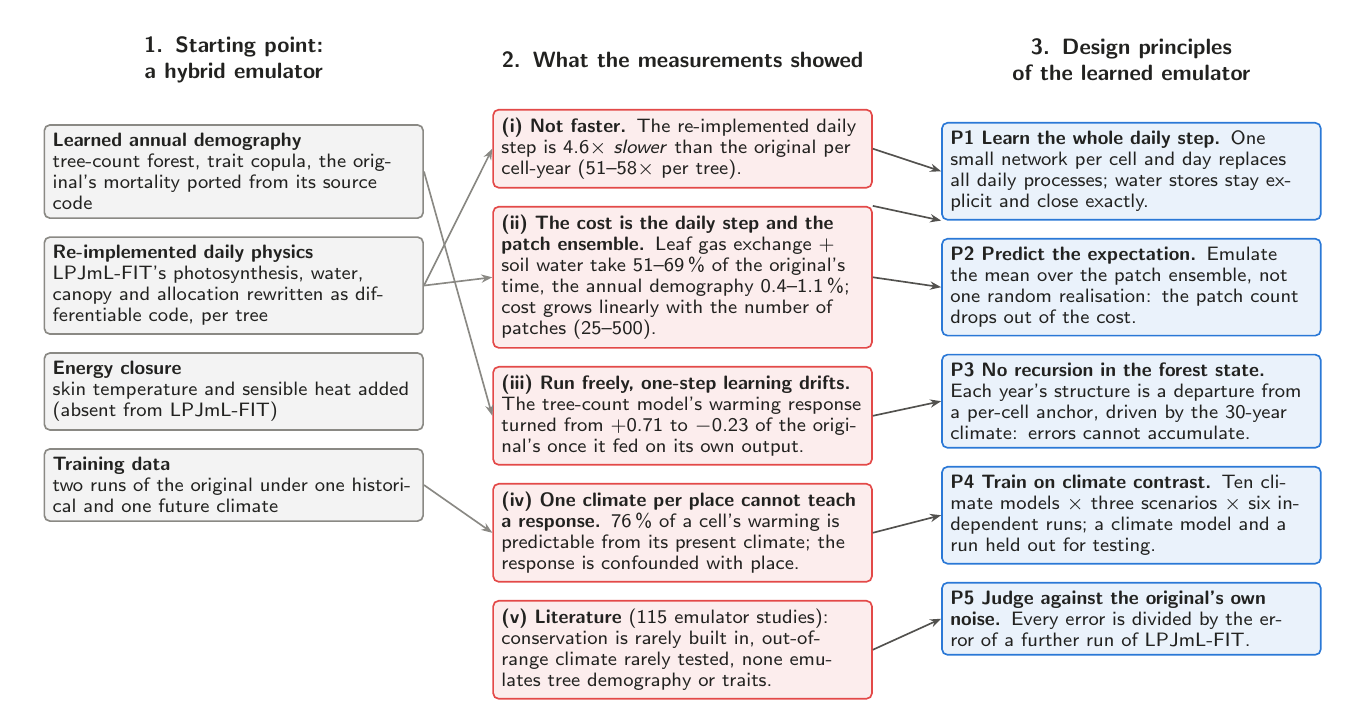
\begin{tikzpicture}[node distance=2.2mm]
% column headers
\node[h] (h1) at (0,0) {1. Starting point:\\ a hybrid emulator};
\node[h] (h2) at (57mm,0) {2. What the measurements showed};
\node[h] (h3) at (114mm,0) {3. Design principles\\ of the learned emulator};

% column 1
\node[b=grey, below=4mm of h1] (c1a) {\textbf{Learned annual demography}\\ tree-count forest, trait copula,
  the original's mortality ported from its source code};
\node[b=grey, below=of c1a] (c1b) {\textbf{Re-implemented daily physics}\\ LPJmL-FIT's photosynthesis, water,
  canopy and allocation rewritten as differentiable code, per tree};
\node[b=grey, below=of c1b] (c1c) {\textbf{Energy closure}\\ skin temperature and sensible heat added
  (absent from LPJmL-FIT)};
\node[b=grey, below=of c1c] (c1d) {\textbf{Training data}\\ two runs of the original under one
  historical and one future climate};

% column 2 (ordered to face the principle each lesson motivates)
\node[b=red, below=4mm of h2] (l1) {\textbf{(i) Not faster.} The re-implemented daily step is
  4.6$\times$ \emph{slower} than the original per cell-year (51--58$\times$ per tree).};
\node[b=red, below=of l1] (l3) {\textbf{(ii) The cost is the daily step and the patch ensemble.}
  Leaf gas exchange + soil water take 51--69\,\% of the original's time, the annual demography 0.4--1.1\,\%;
  cost grows linearly with the number of patches (25--500).};
\node[b=red, below=of l3] (l2) {\textbf{(iii) Run freely, one-step learning drifts.} The tree-count
  model's warming response turned from +0.71 to $-$0.23 of the original's once it fed on its own output.};
\node[b=red, below=of l2] (l4) {\textbf{(iv) One climate per place cannot teach a response.}
  76\,\% of a cell's warming is predictable from its present climate; the response is confounded with place.};
\node[b=red, below=of l4] (l5) {\textbf{(v) Literature} (115 emulator studies): conservation is rarely
  built in, out-of-range climate rarely tested, none emulates tree demography or traits.};

% column 3
\node[b=emu, below=4mm of h3] (p1) {\textbf{P1 Learn the whole daily step.} One small network per cell and
  day replaces all daily processes; water stores stay explicit and close exactly.};
\node[b=emu, below=of p1] (p2) {\textbf{P2 Predict the expectation.} Emulate the mean over the patch
  ensemble, not one random realisation: the patch count drops out of the cost.};
\node[b=emu, below=of p2] (p3) {\textbf{P3 No recursion in the forest state.} Each year's structure is a
  departure from a per-cell anchor, driven by the 30-year climate: errors cannot accumulate.};
\node[b=emu, below=of p3] (p4) {\textbf{P4 Train on climate contrast.} Ten climate models $\times$
  three scenarios $\times$ six independent runs; a climate model and a run held out for testing.};
\node[b=emu, below=of p4] (p5) {\textbf{P5 Judge against the original's own noise.} Every error is
  divided by the error of a further run of LPJmL-FIT.};

\draw[arr] (l1.east) -- (p1.west);
\draw[arr] (l3.east) -- (p2.west);
\draw[arr] (l3.north east) -- (p1.south west);
\draw[arr] (l2.east) -- (p3.west);
\draw[arr] (l4.east) -- (p4.west);
\draw[arr] (l5.east) -- (p5.west);
\draw[arr, draw=grey] (c1b.east) -- (l1.west);
\draw[arr, draw=grey] (c1b.east) -- (l3.west);
\draw[arr, draw=grey] (c1a.east) -- (l2.west);
\draw[arr, draw=grey] (c1d.east) -- (l4.west);
\end{tikzpicture}
\end{document}
